\section{Benchmarks}
\label{sec:bench}

We now compare the performance of our implementations following two directions.
First, we compare the successive algorithmic refinement using the \haskell
implementation presented in \cref{sec:motivation} and \cref{sec:improvements}.
We then compare different data-structure implementation for segments
using the \ocaml implementation detailed in \cref{sec:ocaml}.

\subsection{Comparing algorithms in the \haskell implementation}

\cref{sec:motivation} and \cref{sec:improvements} present successive
algorithmic improvements for our language generator. We now evaluate
the impact of these improvements on performances.
The performances are obviously highly dependent on the regular expression
considered. We chose three regular expressions that highlight
the various strength and weaknesses of the different approaches:
\begin{itemize}
\item$\Rstar a$: The \code{star} operation is very performance intensive.
  The input language only contains one segment, which highlight the usefulness
  of sparse indexing and maps. Since each segment of the output language contains
  only one element, this also tests the behavior of star at high length.
\item $\Rstar{(\Rconcat{a}{\Rstar{b}})}$: On the oposite end of the spectrum, this
  regular expression applies \code{star} to a language where all segments
  are neither empty nor full. This measures the performances of \code{star}
  and \code{concatenation} on non-sparse languages.
\item $\Rconcat{\Rcomplement{(\Rstar{a})}}{b}$: Finally, this regular expressions
  tests the generation of a very big language through \code{star} and the
  concatenation to a much smaller language.
\end{itemize}

\TODO{Describe what are the different haskell implementations: naive, ref, seg, refConv, segConv}

The results can be seen in \cref{bench:haskell:all}.
To evaluate the performance, we iterate through the stream of words produced by
the generator and register the time since the start of the iteration
every 20 words. We stop after 5 seconds. We then graph the number reached in
function of the time spent: the faster a curve grows, the faster it generate
words.
We first note that most implementation generates between 3000 and
150000 words in the first second, which is more than sufficient for testing
purposes.
Additionally, the refConv implementation
which uses symbolic segments and convolutions
is the most versatile. This validates our improvements
proposed in \cref{sec:improvements}.
Looking at each graph in more details, we can make the following remarks:
\begin{itemize}[leftmargin=*]
\item All implementations are equally fast on $\Rstar a$ except
for the naive implementation. This is not surprising, since it does not uses
sparse indexing and relies on list lookups.
\item 
For $\Rstar{(\Rconcat{a}{\Rstar{b}})}$ and
$\Rconcat{\Rcomplement{(\Rstar{a})}}{b}$, some implementations showcase
a shape in ``skewed stairs''. This can be seen as insufficient laziness:
when arriving at a new segment, part of the work is done eagerly which causes
a plateau. When that part is done, the enumeration proceeds lazily.
Since laziness and GHC-optimizations are hard to control in a manual fashion,
we did not attempt to correct this.
\item $\Rconcat{\Rcomplement{(\Rstar{a})}}{b}$ demonstrates that sparse indexing
  does degrade performances when applying \code{star} to non-sparse languages.
  The performance impact is however recovered using the convolution technique
  presented in \cref{sec:convolution}.
\item \TODO{Explain why ref is faster on $\Rconcat{\Rcomplement{(\Rstar{a})}}{b}$...}
\end{itemize}

\begin{figure}[h]
  \centering
  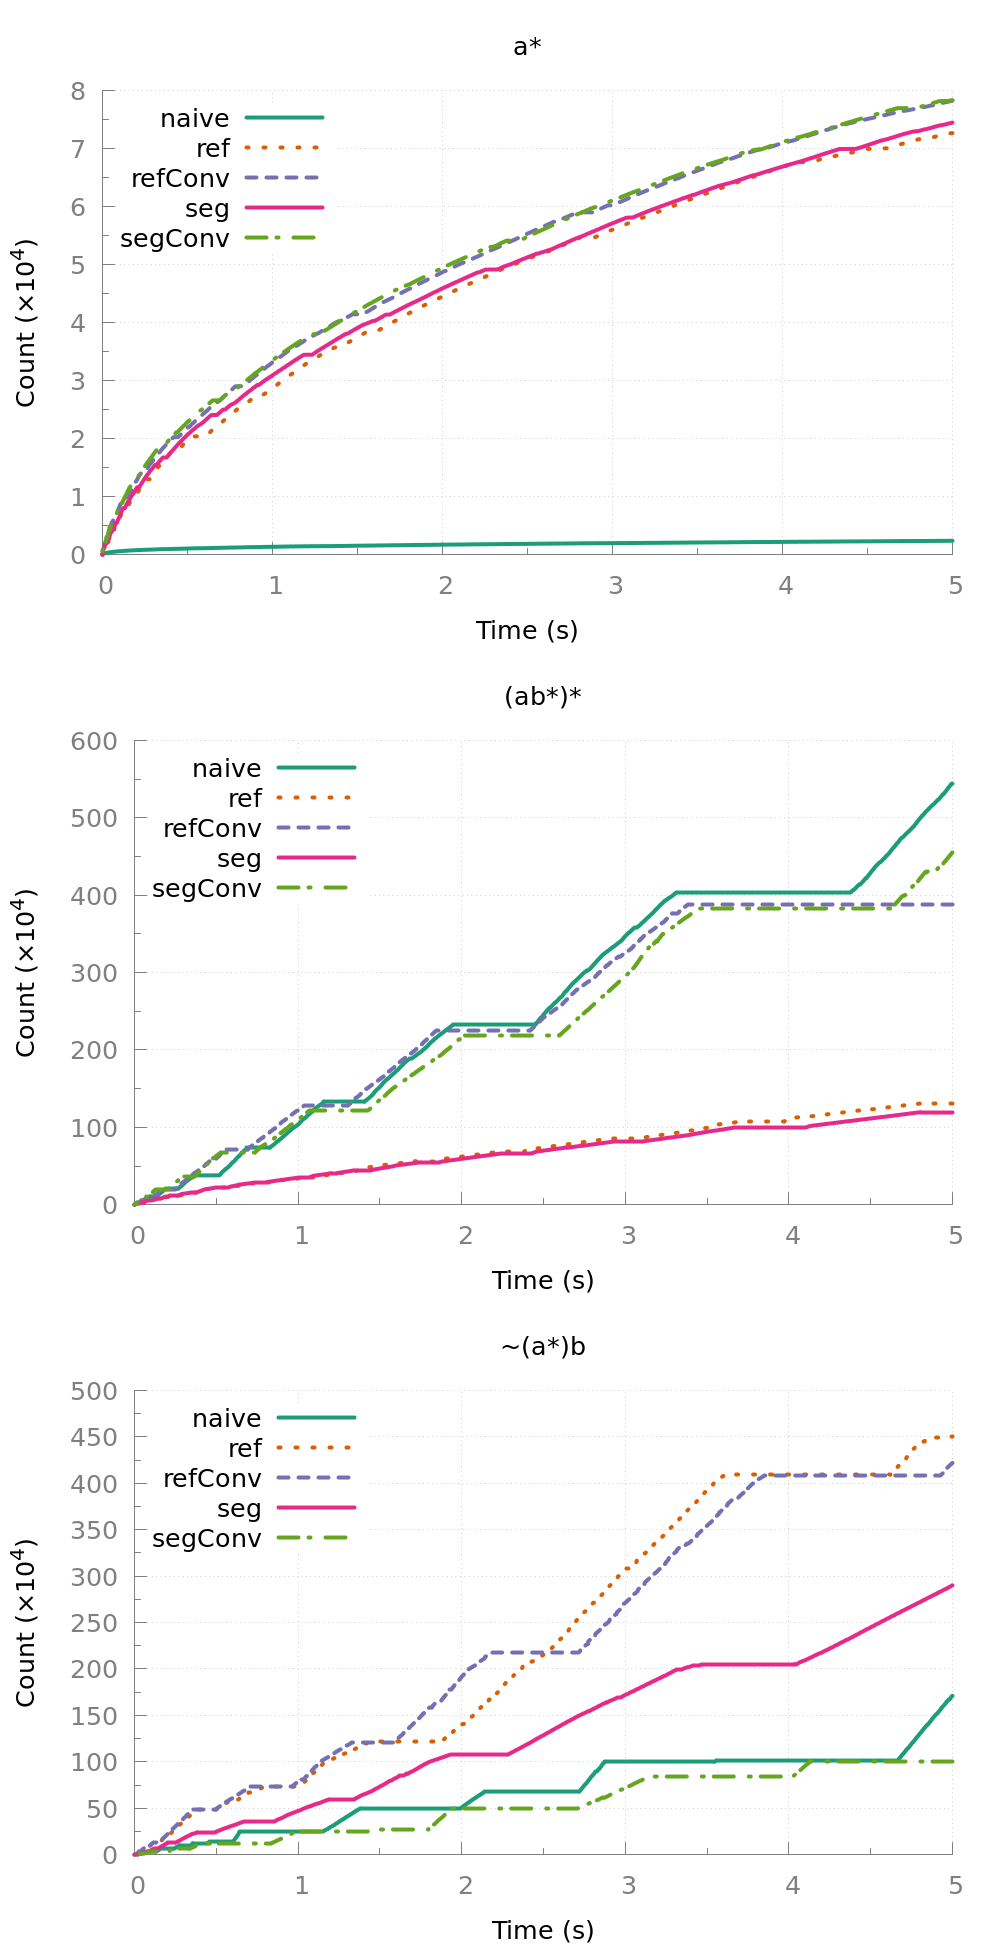
\includegraphics[width=\linewidth]{measure/haskell_all.png}
  \caption{Benchmark for the \haskell implementation with various algorithms}
  \label{bench:haskell:all}
\end{figure}

\subsection{Comparing data-structures in the \ocaml implementation}

We followed the same benchmarking methodology than for the \haskell
version in \autoref{sec:bench}. Benchmark for various data-structures
for regular expressions \verb/a*/, \verb/(ab*)*/ and \verb/~(a*)b/ are
presented in \autoref{bench:ocaml:all}.

\begin{figure}[h]
  \centering
  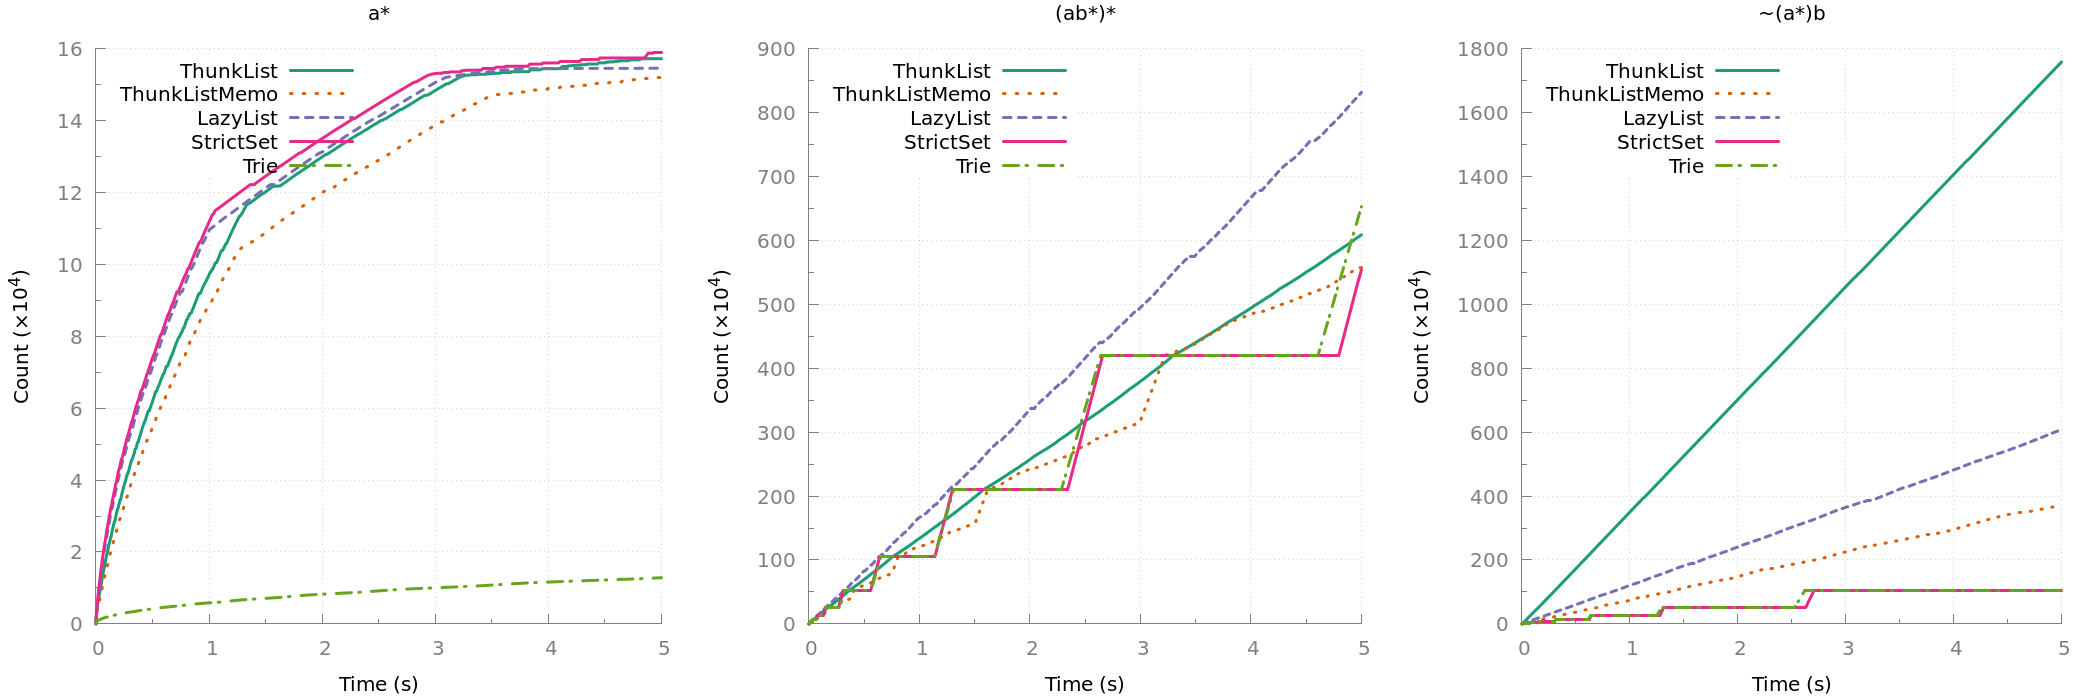
\includegraphics[width=\linewidth]{measure/ocaml_all.png}
  \caption{Benchmark for the \ocaml implementation with various data-structures}
  \label{bench:ocaml:all}
\end{figure}

\subsubsection{Union and set operations}

\begin{figure}[h]
  \centering
  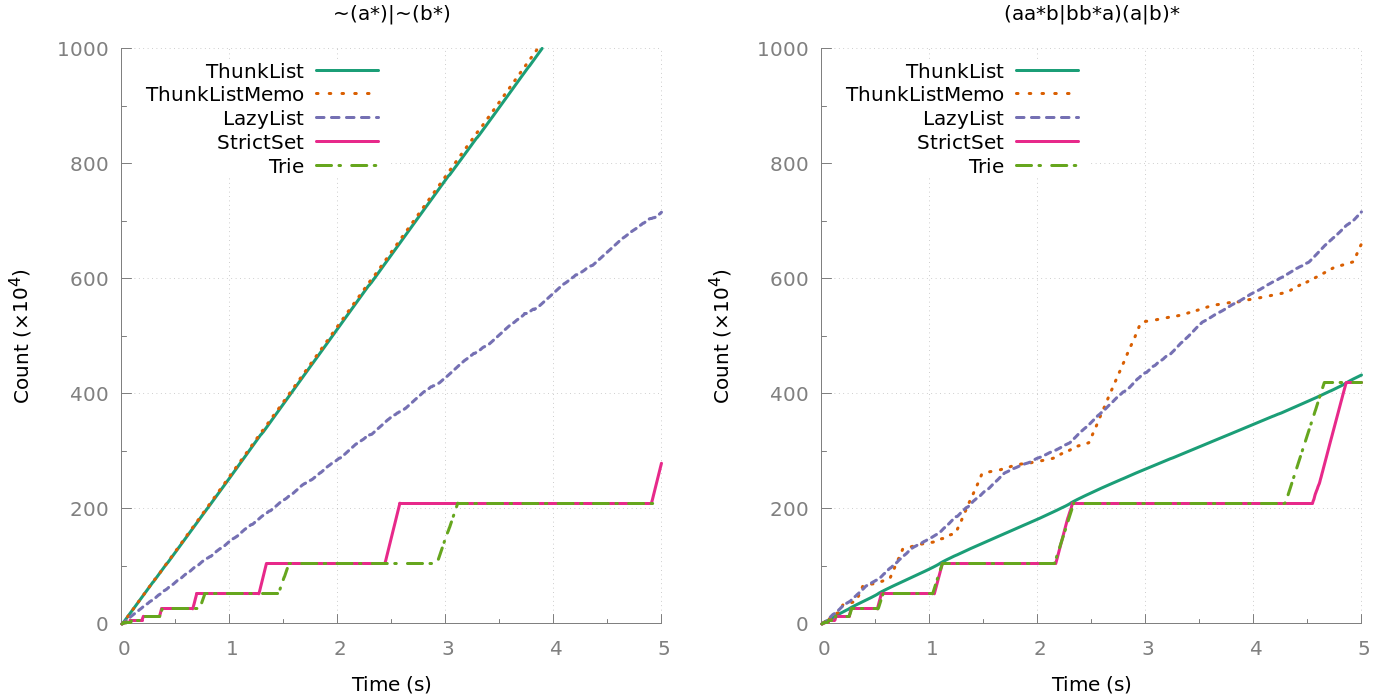
\includegraphics[width=\linewidth]{measure/ocaml_union.png}
  \caption{Benchmarking \texttt{union} in the \ocaml data-structures}
  \label{bench:ocaml:union}
\end{figure}

\subsection{The influence of regular expressions on performances}


\begin{figure}[h]
  \centering
  \begin{subfigure}{0.5\linewidth}
    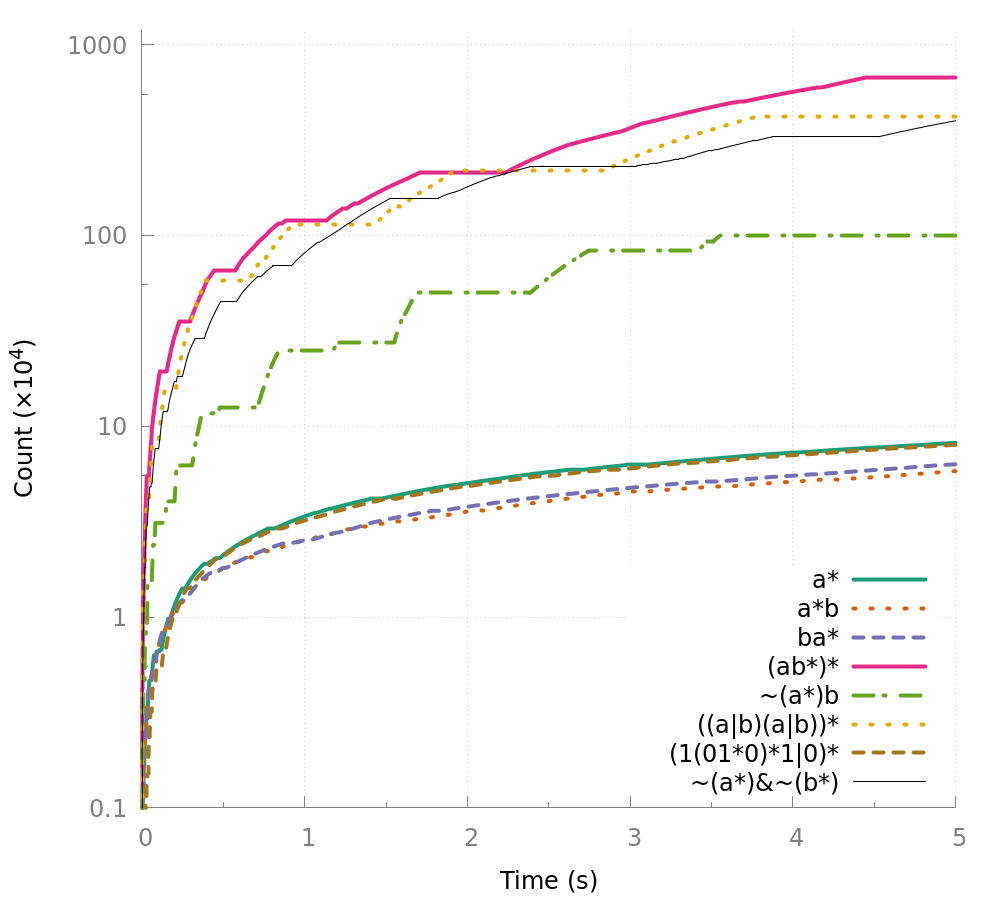
\includegraphics[width=\linewidth]{measure/haskell_langs.png}
    \caption{\haskell implementation with \code{segConv}}
    \label{bench:haskell:langs}
  \end{subfigure}~
  \begin{subfigure}{0.5\linewidth}
    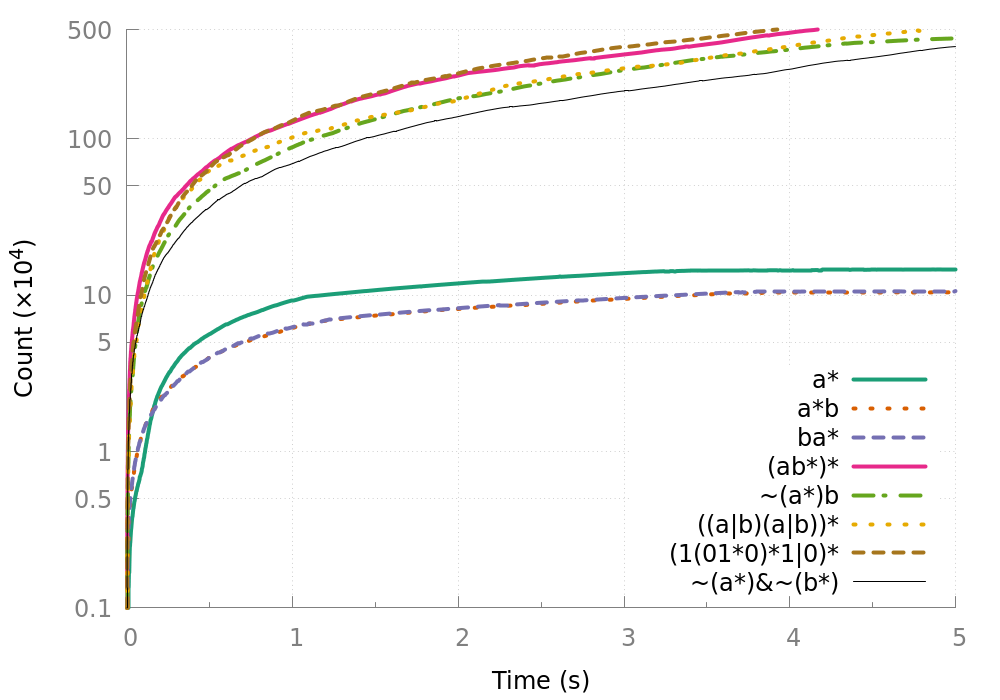
\includegraphics[width=\linewidth]{measure/ocaml_langs.png}
    \caption{\ocaml implementation with \code{ThunkList}}
    \label{bench:ocaml:langs}
  \end{subfigure}
  \caption{Benchmark on different regular expressions}
  \label{bench:langs}
\end{figure}

%%% Local Variables:
%%% mode: latex
%%% TeX-master: "main"
%%% End:
